\chapter{Natural Transformations}

Similar to how morphisms define relations between objects in a category, natural transformations
define relations between functors.
The term ``natural'' in natural transformations was coined by Eilenberg and MacLane (the founders
of Category Theory) due to the fact that these transformations were developed with the
aim of explaining why some constructions in Mathematics were ``natural'' while others
were not.


\section{Defining Natural Transformations}

Similar to functors, the formal definition of natural transformations
are somewhat obscure at first sight, by as we dig a bit, we see that the is
some intuition behind it that makes it easier to understand it.

\begin{definition}[Natural Transformations]
	Let $\mathcal C$ and $\mathcal D$ be categories, and let $F,G:\mathcal C \to \mathcal D$ be functors.
	A natural transformation $\alpha: F \Rightarrow G$ is such that:
	\begin{enumerate}[(i)]
		\item For all $A \in \mathcal C$, there exists $\alpha_A :F(A) \to G(A)$ that is
		      a morphism in $\mathcal D$, i.e $\alpha_A \in Mor_\mathcal D (F(A), G(A))$;
		\item (Naturality) For all $f \in Mor_\mathcal C (A,B)$, then
		      \begin{displaymath}
			      F(f)\fatsemi \alpha_B = \alpha_A \fatsemi G(f).
		      \end{displaymath}

		      Remember that for a morphism $f:A \to B$, we have that $F(f):F(A)\to F(B)$ and $G(f):G(A) \to G(B)$.
		      Since $\alpha_A: F(A) \to G(A)$ and $\alpha_B : F(B) \to G(B)$, then $F(f)$ composes
		      with $\alpha_B$ and $G(f)$ composes with $\alpha_A$, and our definition above works.
	\end{enumerate}
	\label{def:NaturalTransformation}
\end{definition}

Another way to represent property (ii) in the definition of natural transformations
is to affirm that the diagram below.

\begin{figure}[H]
	\begin{center}
		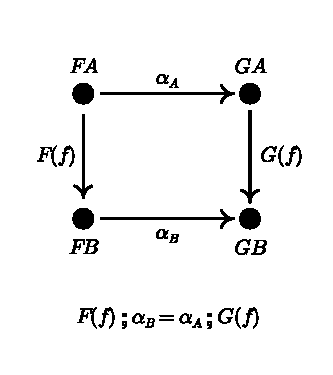
\includegraphics{./notebooks/NaturalTransformation.pdf}
	\end{center}
	\caption{Commutative diagram of a natural transformation highlighting the commutative property of the definition.}
	\label{fig:NaturalTransformation}
\end{figure}

From the definition, the natural transformation $\alpha$ is a transformation between functors
that is in some sense associative, i.e. the order does not matter, we can apply $\alpha$
to $FA$ and then apply $Gf$, or we can apply $Ff$ to $FA$ an then apply the natural transformation. Both
return the same result.

\section{The Category of Functors}

For two categories $\mathcal C$ and $\mathcal D$, we are now tempted to construct a category
where the objects are functors from $\mathcal C$ to $\mathcal D$, and the
morphisms are the natural transformation.
Yet, we must be careful. If $\mathcal C$ and $\mathcal D$ are not small, the
class of objects of each category is not a set, and thus, we cannot
prove the existence of a set of natural transformations between
two functors \citep{borceux1994handbook}.

Fortunately, if $\mathcal C$ is small, this problem goes away, and
we can define such category.

\begin{definition}[Category of Functors]
	For a small category $\mathcal C$ and a category $\mathcal D$,
	$\mathcal D^{\mathcal C}$ is the category of functors
	from $\mathcal C$ to $\mathcal D$ where the morphisms are natural transformations,
	i.e.
	\begin{displaymath}
		Ob_{\mathcal D^{\mathcal C}} :={\text{Functors from } \mathcal C \text{ to } \mathcal D}
	\end{displaymath}
	\begin{displaymath}
		Mor_{\mathcal D^{\mathcal C}}(F,G) :={\text{Natural Transformations from }
		F \text{ to } G}.
	\end{displaymath}
\end{definition}

Since natural transformations are morphisms between functors in this category of functors,
we can now ponder what would an isomorphism between natural transformations look like.
Remember the definition of a categorical isomorphism \ref{def:CategoricalIsomorphism}.

\begin{definition}[Natural Isomorphism]
	Let $\mathcal C$ and $\mathcal D$ be two categories. Two functors
	$F:\mathcal C \to\mathcal D$ and $G:\mathcal C \to\mathcal D$
	are naturally isomorphic if they are isomorphic in the category $\mathcal D^\mathcal C$.
\end{definition}

\begin{theorem}[Natural Isomorphism \citep{spivak2014category}]
	Let $\mathcal C$ and $\mathcal D$ be categories, and $F,G:\mathcal C \to \mathcal D$ functors.
	A natural transformation $\alpha : F \to G$ is an isomorphism in $\mathcal D^\mathcal C$
	if and only if $\alpha_c: F(c) \to G(c)$ is an isomorphism in $\mathcal D$ for every
	$c \in Ob_\mathcal C$.
\end{theorem}
\begin{proof}
	Check proposition 5.3.2.12 from \citet{spivak2014category}.
\end{proof}


\begin{example}[Natural Transformations in Sets]
	Consider the categories $\bm 1$ and $\mathbf{Set}$. We wish to
	construct the category $\mathbf{Set}^{\bm 1}$, i.e. of functors from $\bm 1$
	to $\mathbf{Set}$. Since $\bm 1$ has only one object $1$ and one morphisms $id_1$, then each functor
	$F:\bm 1 \to \mathbf{Set}$ is completely defined by $F(1) = S$, where $S$ is a set, and,
	by the definition of a functor, $F(id_1) = id_S$. This means that every functor
	can be indexed by the set to which it takes the object of $\bm 1$, e.g. $F_A$ is the
	functor that $F_A(1)$ is equal to set $A$.

	Next, we want to define a natural transformation $\alpha: F_A \Rightarrow F_B$.
	By definition, there are two criteria to satisfy. First,
	for every object $1 \in Ob_{\bm 1}$ we have
	$\alpha_1:F_A(1) \to F_B(1)$ such that $\alpha_1 \in Mor_{\mathbf{Set}}(F_A(1),F_B(1))$.
	Since the only object in $\bm 1$ is $1$, we only need to define $\alpha_1$ to fully define $\alpha$.
	Since $\alpha_1$ must be a morphism of $\mathbf{Set}$, then $\alpha_1$ is a function
	from $A$ to $B$.

	Secondly, for every $f \in Mor_{\bm 1} (1,1)$, it's required that
	\begin{displaymath}
		F_A(f) \fatsemi \alpha_1 = \alpha_1 \fatsemi F_B(f).
	\end{displaymath}
	Again, since the only morphism in $\bm 1$ is $id_1$, we only need to prove that
	\begin{displaymath}
		F_A(id_1) \fatsemi \alpha_1 = \alpha_1 \fatsemi F_B(id_1).
	\end{displaymath}

	Note that $F_A(id_1) = id_A$ and $F_B(id_1) = id_B$, and by the definition
	of the identity, we have that for $g \in Mor(A,B)$, $id_A \fatsemi g = g \fatsemi id_B$.
	Hence, the second condition is trivially satisfied.

	With this, we conclude that the natural transformations from
	functors $F_A$ to $F_B$ are, in a sense, isomorphic to functions from sets
	$A$ to $B$.

	Considering the category $\mathbf{SmCat}$ of small categories, we can actually prove
	that $\mathbf{Set}$ and $\mathbf{Set}^{\bm 1}$ are isomorphic.

	Consider the functor
	$I:\mathbf{Set}^{\bm 1} \to \mathbf{Set}$ where $I(F_A) = A \in \mathbf{Set}$ and
	for any natural transformation $\alpha^{(f)}$ where $\alpha^{(f)}_1 = f$, we have
	$I(\alpha^{(f)}) = f$. Also, define $I^{-1}(A) = F_A$ and
	$I^{-1}(f) = \alpha_f$.
	Thus, $I$ defines an isomorphism between the two categories.

\end{example}

\section{Equivalence Between Categories}

We've used the existence of two functors $F:\mathcal C \to \mathcal D$ and $G:\mathcal D \to \mathcal C$,
where $F \fatsemi G = id_\mathcal D$ and $G \fatsemi F = id_\mathcal C$,
to define that two categories are equivalent up to an isomorphism.
Note that in the category of small categories, besides morphisms and objects we also
have natural transformations. Thus, we can make use of natural transformations to
define a new notion of equivalence between categories that is less strict then
the existence of isomorphic functors.

\begin{definition}[Equivalence of Categories]
	We say that a functor $F:\mathcal C \to \mathcal D$ defines an equivalence of
	categories if there exists another functor $G:\mathcal D \to \mathcal C$ and
	two natural transformations
	$\alpha: id_\mathcal C \to G \circ F$ and
	$\beta: id_\mathcal D \to F \circ G$, where $\alpha$ and $\beta$ are natural isomorphisms,
	i.e. for any $c \in \mathcal C$,
	$\alpha_c:id_\mathcal C(c) \to (G \circ F)(c)$ is an
	isomorphism in $\mathcal C$, and for any $d \in \mathcal D$,
	$\beta_d:id_\mathcal D(d) \to (F \circ G)(d)$ is an isomorphism in $\mathcal D$.

	Moreover, we say that $F$ are $G$ are mutually inverse equivalences.
	\label{def:EquivalenceCategories}
\end{definition}

The above definition is convoluted, so let's try to get some intuition.
First, note that $id_\mathcal C(c) = c \in \mathcal C$, so the natural transformation
$\alpha$ defines for each object $c \in \mathcal C$ a morphism $\alpha_c$ from $c$
to $c' = G(F(c)) \in \mathcal C$, where $c$ and $c'$ are actually isomorphic.

Now it's a bit clearer what is going on. The definition is stating that two
categories are equivalent if there is a pair of functors which are almost the inverse
of one another, but instead of $(F \circ G)(c) = c$ we have that
$(F \circ G )(c) = c'$  where $c'$ is isomorphic to $c$.
Thus, our functors are not inverses, because they scramble the objects, but in the end,
they just exchange objects that are isomorphic to one another, hence, they ``keep everything
almost the same''.

\section{Vertical vs Horizontal Compostion}

We already introduced how we compose natural transformations in
a category of functors $\mathcal D^{\mathcal C}$. This composition
is referred by \citet{spivak2014category} as \textit{vertical}, because
it can be depicted by the Figure below.

Yet, there is another type of operation between natural transformations,
called \textit{Whiskering}, also referred as \textit{horizontal composition}
by \citet{spivak2014category}. This time, the name is inspired by
the diagram below.

\begin{definition}[Prewhiskering]
	Let $\mathcal B, \mathcal C, \mathcal D$ be categories, and define
	functors $G_1,G_2:\mathcal C \to \mathcal D$,
	$F:\mathcal B \to \mathcal C$ and the natural transformation
	$\alpha: G_1 \to G_2$.
	A \textit{postwhiskering}
	of $\alpha$ by $\mathcal G$ is denoted by $\alpha \diamond G:G_1 \circ F \to G_2 \circ F$,
	where for every $b \in Ob_\mathcal B$, $(\alpha \diamond F)_b:(G_1 \circ F)(b) \to (G_2 \circ F)(b)$
	is defined to be $\alpha_{F(b)}$
	\label{def:prewhiskering}
\end{definition}

\begin{definition}[Postwhiskering]
	Let $\mathcal B, \mathcal C, \mathcal D$ be categories, and define
	functors $F_1,F_2:\mathcal B \to \mathcal C$,
	$G:\mathcal C \to \mathcal D$ and the natural transformation
	$\beta F_1 \to F_2$.
	A \textit{postwhiskering}
	of $\beta$ by $\mathcal G$ is denoted by $G \diamond \beta:G \circ F_1 \to G \circ F_2$,
	where for every $c \in Ob_\mathcal C$, $(\beta \diamond G)_b:(G \circ F_1)(c) \to (G \circ F_2)(c)$
	is defined to be $G(\beta_c)$ .
	\label{def:postwhiskering}
\end{definition}

From these definitions of prewhiskering and postwhiskering, we construct the Whiskering,
which is just the composition of a prewhiskering with a postwhiskering.

\begin{definition}[Horizontal Composition/Whiskering of Natural Transformations]
	Let $\mathcal B, \mathcal C, \mathcal D$ be categories, and define
	functors $F_1,F_2:\mathcal B \to \mathcal C$ and
	$G_1, G_2 :\mathcal C \to \mathcal D$. For two natural transformations
	$\alpha: G_1 \to G_2$ and $\beta: F_1 \to F_2$,
	a \textit{whiskering} (horizontal composition)
	is denoted by
	$\alpha \diamond \beta: G_1\circ F_1 \rightarrow G_2 \circ F_2$
	where:
	\begin{displaymath}
		\alpha \diamond \beta
		= (\alpha \diamond F_1) \circ (G_2 \diamond \beta)
		= (G_1 \diamond \beta) \circ (\alpha \diamond G_2).
	\end{displaymath}
	\label{def:Whiskering}
\end{definition}

\begin{theorem}[Interchange for Whiskering]
	(image here)

	Given the setup above, then we have
	\begin{displaymath}
		(\beta_2 \circ \beta_1) \diamond (\alpha_2 \circ \alpha_1) =
		(\beta_2 \diamond \alpha_2) \circ (\beta_1 \diamond \alpha_1).
	\end{displaymath}

\end{theorem}
